
\chapter[Ontology of attribution marking]{An ontology of adjective attribution marking devices}
The previous sections of this chapter were aimed at typologizing adjective attribution marking devices. The attested devices described so far belong to the following noun phrase types:
\begin{itemize}
\item{Juxtaposition}
\item{Incorporation}
\item{Construct state}
\item{Linker}
\item{Anti-construct state}
\item{Attributive nominalization}
\item{Attributive article}
\item{Anti-construct state agreement}
\item{Head-driven agreement}
\item{Apposed head-driven agreement}
\item{Modifier-headed possessor agreement}
\end{itemize}
Table \ref{tabledefontology} on page \pageref{tabledefontology} summarizes the typology from the previous chapter and presents short definitions (including bracketed syntactic templates) and an example for each type.\footnote{This overview is derived from the definition file of general noun phrase patterns included in \citet{AUTOTYP-NP}.} Note that a lexical head is required only in certain noun phrase types. Note also that the constituent order (e.g. [$_{NP}$ A N] or [$_{NP}$ N A]) and the morpho-phonological fusion of formatives (e.g. (free) [$_{NP}$ A \textsc{nmlz}], (cumulative) [$_{AP}$ A:\textsc{attr:agr}] or (affixal) [$_{AP}$ A-\textsc{attr}]) is not relevant for the presented ontology.\footnote{The presented ontology is defined by (mostly) morpho-syntactic parameters. But grammatical word-hood could be relevant for definitions of subtypes in the leaves of Figure \ref{tree ontology}. For instance {\it head-driven agreement} could perhaps be sub-divided into types exhibiting agreement affixes vs. grammatical agreement words.}

Table \ref{syntaxontology} on page \pageref{syntaxontology} presents an ontological cross-classification of all devices defined earlier. This ontology has three main dimensions: 
\begin{itemize}
\item{{\it Syntactic source}}, i.e.~the central syntactic operation which constitutes attribution and belongs either to {\it agreement marking} or {\it government}. But note that syntactic government can include secondary, i.e.~non-constitutional agreement.
\item{{\it Syntactic pattern}}, i.e.~devices projecting adjective phrases versus devices projecting full noun phrases (by means of attributive apposition or, in the case of modifier-headed possessor agreement, by converting the attribute to the “possessed” noun phrase).
\item{The {\it Syntactic locus}} of the respective formatives.
\end{itemize}
Figure \ref{tree ontology} on page \pageref{tree ontology} presents a similar ontology in a tree diagram. The order of types (from left to right) is similar to Table \ref{tabledefontology} (from top to bottom). The left branch of the tree consists of a purely syntactic device ({\it juxtaposition}) with the subtype ({\it incorporation}); the middle branch consists of three overt morpho-syntactic types differentiated by the locus of the respective formatives: on-head ({\it construct state}), floating ({\it linker}) and on-dependent. “Dependent-marking” a\-gain can be divided further into the three subtypes: {\it attributive nominalization}, {\it anti-construct state agreement} and {\it attributive article} (a subtype of {\it attributive nominalization}). The right branch of the tree, finally, comprises morpho-semantico-syntactic devices, i.e. devices primarily connected to head- ({\it head-driven agreement}) or dependent-driven agreement ({\it modifier-headed possessor agreement}). A dashed line combines the types of {\it head-driven agreement}, {\it anti-construct state agreement} and {\it attributive article} because (morpho-semantico-syntactic) agreement marking is involved in all of them.

Whereas construct- and agreement marking in the types of {\it anti-construct state agreement} and {\it attributive article} are combined in portmanteau morphemes (e.g.~in the anti-construct state agreement marking suffixes in Russian) other devices can (or must) co-occur without being combined into one formative. Attested and non-attested combinations of adjective attribution marking devices are illustrated in Table \ref{nichtkombiniert}.
The attested co-occurring adjective attribution marking devices are:
\begin{itemize}
\item{Anti-construct state agreement + Head-driven agreement (“Double agreement”)}
\item{Anti-construct state + construct state (“Double construct”)}
\item{Anti-construct state + attributive article (“Double construct”)}
\item{Attributive article + head-driven agreement (“Double agreement”)}
\end{itemize}

\begin{table}
\begin{footnotesize}
\begin{center}
\begin{tabular}{l | l | l}
\hline
\hline
Device 1 & Device 2 & Note\\
\hline
Juxt & – & No logical combination possible\\
Inc & ? & No attestation of any combination\\ 
Constr &AConstr &  Northern Saami (“Double construct”)\\
Nmlz (Art) & AConstr & Endo (“Double construct”)\\
ACAgr  & HDAgr & Swedish (“Double agreement”)\\
Nmlz (Art)&HDAgr & Albanian (“Double agreement”)\\
Link & ? & No attestation of any combination\\
MHPAgr & ? & No attestation of any combination\\ 
\hline
\hline
\end{tabular}
\end{center}
\end{footnotesize}
\caption[Attested combined devices]{Attested combined adjective attribution marking devices} \label{nichtkombiniert}
\end{table}

\begin{landscape}
\begin{table}
\begin{footnotesize}
\begin{center}
\begin{tabular}{l l l l l}
\hline
\hline
Type	&Definition&Syntactic&Common&Example\\
	&		&dependency&label&language\\
\hline
\hline
Juxt		&Unmarked sequence of constituents; Test:&$[_{NP} [_{AP}$ A$]$ (N)$]$&Juxtapo-&Komi	\\
		& no additional morphemes available in NP&&sition\\
\hline
Inc		&No additional morphemes available in NP, but dep is syntactic&$[_{NP}$ A-N$]$&Incorpo-&Chukchi\\
		&compound; Test: dep cannot occur unbound (headless)&&ration\\
\hline
Constr	&Head-marking formative that only registers presence of dep; Test: formative does not&$[_{NP} [_{AP}$ A (N:\textsc{attr})$] ]$&Ezafe&Kurmanji\\
		& undergo agreement and is not present without head (in predication) or without dep\\
\hline
Link	&Floating formative (neither ad-head nor ad-dep, but truly ad-&$[_{NP} [_{AP}$ A] \textsc{attr} N$]$&Linker&Tagalog\\
		&phrase) that only registers presence of head-dep relation; Test: for-\\
		&mative not present without head (in predication) or without dep\\
\hline
AConstr	&Dep-marking formative that only registers presence of head; Test: formative &$[_{NP} [_{AP}$ A:\textsc{attr}$]$ (N)$]$&Attributive&Saami\\
		&does not undergo agreement and is not present without head (in predication)&& suffix\\
\hline
Nmlz		&Dep-marking formative that only registers presence of head by projec- &$[_{NP} [_{NP} [_{AP}$ A\textsc{:nmlz}$] ]$ (N)$]$&Nominalizer&Udmurt\\
		&ting full NP; Test: formative does not undergo agreement and is used\\
		&in focus construction where inflection of the head is reduplicated\\
\hline
Art		&Subtype of nominalizer &$[_{NP} [_{NP} [_{AP}$ A \textsc{nmlz:agr}$] ]$ (N)$]$&Double&Yiddish\\
		&that undergoes agreement&										&article\\
\hline
ACAgr	&Dep-marking formative that registers presence of head and undergoes agree-&$[_{NP} [_{AP}$ A\textsc{:attr:agr}$]$ (N)$]$&Long-form&Russian	\\
		&ment triggered by the head; Test: not present without head (in predication)&& adjective\\
\hline
HDAgr	&Dep-marking formative that duplicates &$[_{NP} [_{AP}$ A:\textsc{agr}$]$ (N)$]$&Agreement&Finnish\\
		&morpho-semantic features of the head&& suffix\\
		\hline
AHDAgr	&AP marked with HDAgr but projecting a full NP in apposition; &$[_{NP} [_{NP} [_{AP}$ A\textsc{:agr}$]$ (N)$]$&Appositional&Georgian\\
		&Test: AP is used in focus construction where inflection of the && agreement\\
		& head is reduplicated, often with reversed constituent order\\
\hline
MHPAgr	&Head-marking formative that duplicates morpho-semantic features of &$[_{NP} [_{PSD} [ A:\textsc{poss:agr}] (_{PSR}N)]$&Possessive-&Saliba\\
		&(adjectival) dep by means of possessor agreement in a modifier-headed NP&&like attribute\\
\hline
\hline
\end{tabular}
\end{center}
\end{footnotesize}
\caption[Ontology: Definitions]{Attested adjective attribution marking devices with definitions and examples. \textbf{Type abbreviations:} ACAgr=Anti-construct state agreement, AConstr=Anti-construct state, AHDAgr=Appositive head-driven agreement, Art=Attributive article, Constr=Construct state, HDAgr=Head-driven agreement, Inc=Incorporation, Juxt=Juxtaposition, Link=Linker, MHPAgr=Modifier-headed possessor agreement, Nmlz=Attributive nominalization}\label{tabledefontology}
\end{table}

\begin{table}
\begin{footnotesize}
\begin{center}
\begin{tabular}{|| r || c | c | c | c || c | c ||}
\hline
\hline
			&\multicolumn{6}{c||}{Syntactic source}\\

			\cline{2-7}
			&\multicolumn{4}{c||}{{\it Government $[+GOV]$ $[±(Secondary)AGR]$}}&\multicolumn{2}{c||}{{\it Agreement $[-GOV]$ $[+(Primary)AGR]$}}\\
			\cline{2-7}
			&\multicolumn{4}{c||}{Syntactic pattern}&\multicolumn{2}{c||}{Syntactic pattern}\\
			\cline{2-7}
$Locus$		&$[±AGR]$	&Embedded	&Non-embedded			&Incorporated	&Embedded&Non-embedded\\
\hline
\hline	
no			&\textbackslash/&			&{\bf Juxtaposition}						&{\bf Incorporation}			&\textbackslash/&\textbackslash/ \\
marking		&/\textbackslash&			&[$_{NP}$ A (N)]				&[$_{NP}$ A *(N)]&/\textbackslash&/\textbackslash\\
\hline
\hline
			& 			&			&{\bf Linker}						&			&			&\\
floating		&$[–AGR]$	&			&[$_{NP}$ A \textsc{attr} *(N)]	&			&			&\\
 			\cline{2-5}
			&$[+AGR]$	&			&							&			&			&\\
			&			&			&							&			&			&\\
\hline
\hline
			&			&{\bf Nominalization}&{\bf Anti-Construct State}			&	&{\bf Appositive Head-Driven}&{\bf Head-Driven}\\
dep-			&$[–AGR]$	&[$_{NP}$ [$_{NP'}$ A:\textsc{nmlz}] (N)]&[$_{NP}$ A:\textsc{attr} (N)]&&{\bf Agreement}&{\bf Agreement}\\		
			\cline{2-5}
marking		&$[+AGR]$	&{\bf Article}		&{\bf Anti-Construct Agreement}	&			&[$_{NP}$ [$_{NP'}$ A \textsc{agr}] (N)]&[$_{NP}$ A \textsc{agr} (N)]\\
			&&[$_{NP}$ [$_{NP'}$ A:\textsc{nmlz:agr}] (N)]&[$_{NP}$ A:\textsc{attr:agr} (N)]&&&\\
\hline
\hline
			&			&			&{\bf Construct State}						&			&{\bf Modifier-Headed }	&\\
head-		&$[–AGR]$	&			&[$_{NP}$ A *(N:\textsc{attr})]&&{\bf Possessor Agreement}&\\
			\cline{2-5}
marking		&$[+AGR]$	&			&							&&[$_{NP}$ [$_{PSD}$ A:\textsc{poss:agr}] ($_{PSR}$N)]&\\
			&			&			&							&&&\\
\hline
\hline
\end{tabular}
\caption[Ontology: Multidimensional diagram]{Multidimensional ontology of noun phrase structures according to the parameters {\it syntactic source} (true agreement marking or governed [±~additional agreement]) and {\it syntactic pattern} of the device (projects noun phrase, projects adjective phrase) as well as {\it syntactic locus} of the respective markers (on-head, on-dependent, floating). Note that some cells in the table are marked for logically impossible types. \textbf{Type abbreviations:} ACAgr=Anti-construct state agreement, AConstr=Anti-construct state, AHDAgr=Appositive head-driven agreement, Art=Attributive article, Constr=Construct state, HDAgr=Head-driven agreement, Inc=Incorporation, Juxt=Juxtaposition, Link=Linker, MHPAgr=Modifier-headed possessor agreement, Nmlz=Attributive nominalization. {\bf Glosses and tags:} A=Adjective, $AGR$=Agreement, \textsc{agr}=Agreement marker, AP=Adjective phrase, \textsc{attr}=Attribution marker, $GOV$=Government, N=Noun, \textsc{nmlz}=Nominalization marker (Attributive nominalizer), NP=Noun phrase, \textsc{poss}=Possessive marker, PSD=Possessed noun phrase, PSR=Possessor noun phrase}\label{syntaxontology}
\end{center}
\end{footnotesize}
\end{table}

\begin{figure}
\caption[Ontology of adjective attribution marking types]{Ontological tree of attested adjective attribution marking devices} \label{tree ontology}\bigskip
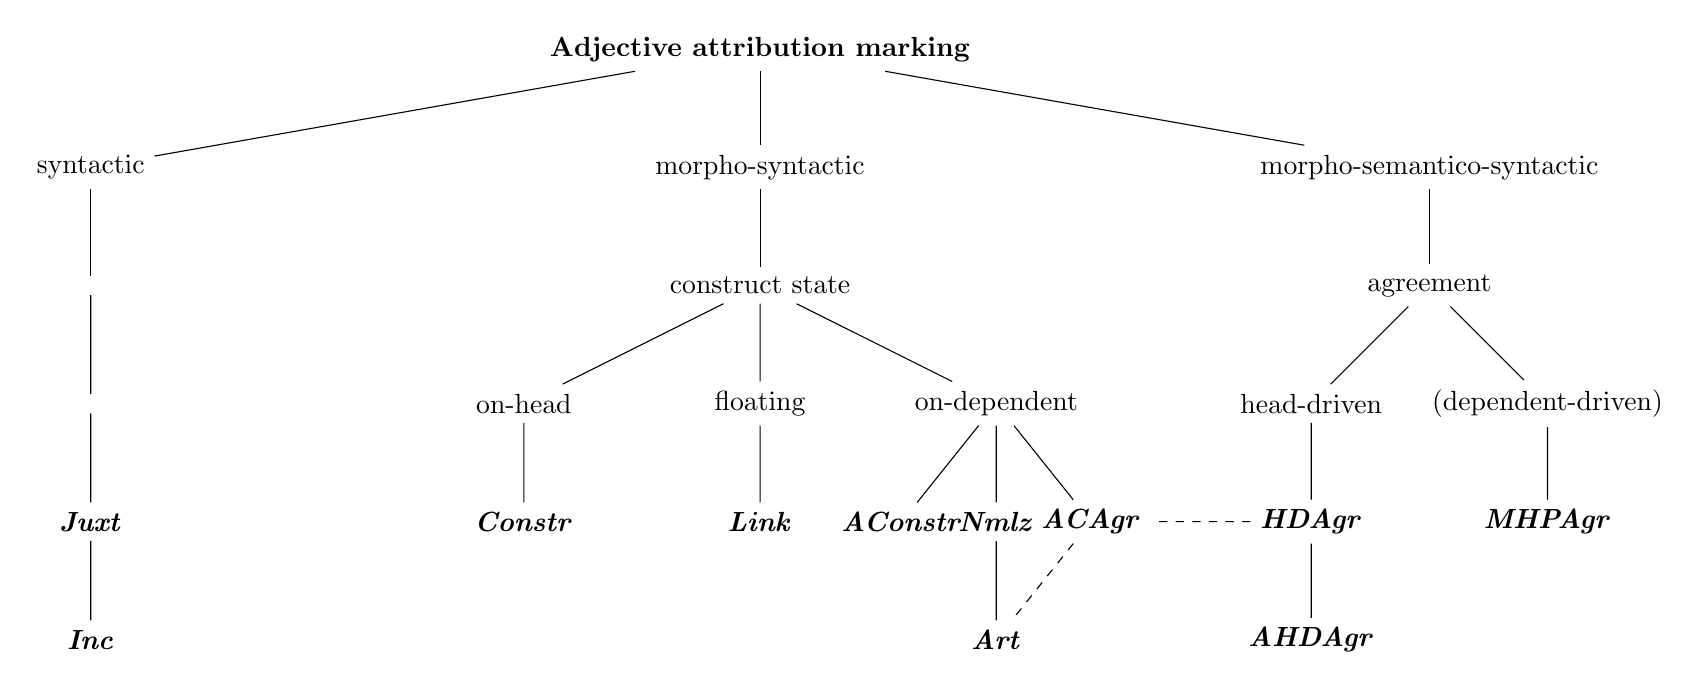
\begin{tikzpicture}
\tikzstyle{level 1}=[sibling distance=85mm]
\tikzstyle{level 3}=[sibling distance=30mm]
\tikzstyle{level 4}=[sibling distance=12mm]
\node {\textbf{Adjective attribution marking}}
child {node {syntactic}
	child {node {}
		child {node {}
			child {node {\textbf{\textit{Juxt}} }
				child {node {\textbf{\textit{Inc}} }
				}
			}
		}
	}
}
child {node {morpho-syntactic}
	child {node {construct state}
		child {node {on-head}
			child{node {\textbf{\textit{Constr}} }
			}
		}
		child {node {floating}
			child{node {\textbf{\textit{Link}} }
			}
		}
		child {node {on-dependent}
			child{node {\textbf{\textit{AConstr}} }
			}
			child{node {\textbf{\textit{Nmlz}} }
				child{node (Art) {\textbf{\textit{Art}} }
				}
			}
			child{node (ACAgr) {\textbf{\textit{ACAgr}} }
			}
		}
	}
}
child {node {morpho-semantico-syntactic}
	child {node {agreement}
		child {node {head-driven}
			child {node (HDAgr) {\textbf{\textit{HDAgr}} }
				child {node {\textbf{\textit{AHDAgr}} }
				}
			}
		}
		child {node {(dependent-driven)}
			child {node {\textbf{\textit{MHPAgr}} }
			}
		}
	}
};
\draw [dashed] (HDAgr) -- (ACAgr) -- (Art);
\end{tikzpicture}
\end{figure}
\end{landscape}
